\documentclass[12pt,a4paper,notitlepage]{article}

\usepackage[utf8]{inputenc}

\usepackage[francais]{babel}\usepackage[T1]{fontenc}
\usepackage[cyr]{aeguill}
\usepackage{lmodern}
\usepackage{color}
\usepackage{boites}
\usepackage{caption}
\usepackage{fancybox}
\usepackage{listings}
%\lstset{language=bash, basicstyle=\footnotesize, frame=shadowbox, rulesepcolor=\color{gris}, captionpos=b}

  \lstset{
         basicstyle=\footnotesize\ttfamily, % Standardschrift
         %numbers=left,               % Ort der Zeilennummern
         numberstyle=\tiny,          % Stil der Zeilennummern
         %stepnumber=2,               % Abstand zwischen den Zeilennummern
         numbersep=5pt,              % Abstand der Nummern zum Text
         tabsize=2,                  % Groesse von Tabs
         extendedchars=true,         %
         breaklines=true,            % Zeilen werden Umgebrochen
         keywordstyle=\color{red},
                frame=b,         
         keywordstyle=[1]{\itshape}{//},    % Stil der Keywords
         stringstyle=\color{white}\ttfamily, % Farbe der String
         showspaces=false,           % Leerzeichen anzeigen ?
         showtabs=false,             % Tabs anzeigen ?
         xleftmargin=5pt,
         framexleftmargin=1pt,
         framexrightmargin=5pt,
         %numbers=left,
         frame=toplines,
         framextopmargin=3pt,
       %  framexleftmargin=8pt,
         numberblanklines=false,
         %morecomment=[s][marron]{/*}{*/},
         %moredelim=*[s][\color{blue}]{/*}{*/}
         %morecomment=[s][marron]{/*-}{*/}},         
         framexbottommargin=5pt,
         captionpos=b,
         %backgroundcolor=\color{lightgray},
         showstringspaces=false      % Leerzeichen in Strings anzeigen ? 
 }

\DeclareCaptionFont{white}{\color{white}}
\DeclareCaptionFormat{listing}{\colorbox[cmyk]{0.43, 0.35, 0.35,0.01}{\parbox{\textwidth}{\hspace{10pt}#1#2#3}}}
\captionsetup[lstlisting]{format=listing,labelfont=white,textfont=white, singlelinecheck=false, margin=0pt, font={bf,footnotesize}}

\definecolor{gris}{gray}{0.75}
%\definecolor{bleup}{HTML}{258EE9}


%\renewcommand*\familydefault{\ttdefault} %% Only if the base font of the document is to be typewriter style
%\renewcommand{\rmdefault}{ptm}


\usepackage[
   pdfauthor={Ludovic Terrier & Arnaud Goulut},
   pdftitle={RE12 - TP2},
   ]{hyperref}
   
   
\usepackage[pdftex]{graphicx}

%\usepackage{titlesec}
%\titleformat{\section}[frame] {\normalfont} {\filright
%\footnotesize
%\enspace\textbf{\thesection}\enspace} {8pt} {\Large\bfseries\filcenter}

%% Je contrôle la taille de ma zone imprimée...
\usepackage{anysize}
%% ...en définissants les marges {gauche}{droite}{haute}{basse}
\marginsize{25mm}{15mm}{10mm}{15mm}

\begin{document}

\title{Mise en \oe uvre d'un annuaire LDAP}
\author{Arnaud Goulut et Ludovic Terrier}
\date{Mai 2010}
\maketitle


%\tableofcontents

\thispagestyle{empty}


%%%%%%%%%%%%%%%%%%%%%%%%%%%%%%%%%%%  1ère page 


%%%%%%%%%%%%%%%%%%%%%%%%%%%%%%%%%%% 1ère partie
\section{Connexion à un annuaire existant}

\subsection{Installation du client LDAP admin tool}
Pour installer le logiciel, on récupère l'archive, et on la décompresse. Ensuite : \\

\noindent \texttt{user@machine  chmod +x LdapAdminTool-4.6.1.x-Linux-x86-Install.bin \\
user@machine  ./LdapAdminTool-4.6.1.x-Linux-x86-Install.bin}
\bigskip


\subsection{Connexion anonyme à un annuaire}
Pour se connecter de manière anonyme à un annuair LDAP, on renseigne les champs :

\begin{itemize}
\item hôte : \textbf{ldap.baylor.edu}
\item DN: \textbf{o=Baylor University, c=US}
\end{itemize}

\bigskip

L'annuaire est organisé selon le modèle pays / organisation. \\

L'objet racine contient :
\begin{itemize}
\item o : pour Organisation, précise le nom de l'organisation : ici Baylor University
\item aci : pour Access Control Item, qui définit le contrôle aux accès pour chaque objet
\item objectclass organization
\item objectclass top
\end{itemize}
\bigskip
Pour un élève on retrouve les informations suivantes :

\begin{itemize}
\item objectclass : baylorperson
\item objectclass : inetorgperson
\item objectclass : organizationalperson
\item objectclass : person
\item objectclass : top
\item cn : Teresa Bennett
\item cn : Teresa Gail Cowan
\item sn : Cowan
\item givenname : Teresa Gail
\item krbname : Teresa-Bennett
\item mail : Theresa-Bennett AT baylor.edu
\item ou : Other
\item ou : People
\item pid : 100004149
\item uid : Theresa-Bennett
\end{itemize}

  
\subsection{Recherche dans un annuaire}
Blablala

\subsection{Exportation LDIF}


\clearpage
\section{Mise en \oe uvre d'un serveur}
%Le serveur
\subsection{Installation d' OpenLDAP}

L'installation du serveur LDAP se fait, en root, via la commande : \texttt{yum install openldap}\\

Après avoir installé le serveur \texttt{openldap} il suffit d'éditer le fichier \texttt{/etc/openldap/slapd.conf} en y ajoutant la partie : 

\begin{lstlisting}[title=Contenu du fichier slapd.conf]
suffix          "dc=musicschool,dc=fr"
rootdn          "cn=admin,dc=musicschool,dc=fr"
rootpw           {SSHA}RqOzsduTTgQX9eVbo1FDHpUaZEIdyd77

\end{lstlisting}

Le champ  \texttt{rootpw} est complété grâce à la commande \texttt{slappasswd} qui permet de générer un hash pour un mot de passe donné. Ceci permet de ne pas laisser le mot de passe administrateur en clair dans le fichier de configuration.\\


\subsection{Peuplement de l'annuaire}
Dans cette partie, nous allons voir comment ajouter et supprimer des utilisateurs de notre annuaire via l'outil \texttt{ldapadd}.\\

Une fois le fichier LDIF créé, on l'ajoute à l'annuaire avec la commande :

\noindent \texttt{ldapadd -x -D "cn=admin,dc=musicschool,dc=fr" -W -f racine.ldif}

\subsubsection{Ajout de la racine}

\begin{lstlisting}[title=racine.ldif]
dn: dc=musicschool,dc=fr
objectClass: dcObject
objectClass: organization
o: Musicschool
description: Une ecole de musique 
dc: musicschool 
\end{lstlisting}


\subsubsection{Ajout de l'OU people}

\begin{lstlisting}[title=people.ldif]
dn: sn=Doussot,ou=people,dc=musicschool,dc=fr
cn: Michel Doussot
objectClass: top
objectClass: inetOrgPerson
sn: Doussot

dn: sn=Ploix,ou=people,dc=musicschool,dc=fr
cn: Alain Ploix
objectClass: top
objectClass: inetOrgPerson
sn: Ploix
\end{lstlisting}

\subsubsection{Ajout de l'OU rôle}

\begin{lstlisting}[title=role.ldif]
dn: ou=roles,dc=musicschool,dc=fr
objectClass: top
objectClass: organizationalUnit
ou: roles

dn: cn=eleves,ou=roles,dc=musicschool,dc=fr
objectClass: groupOfUniqueNames
cn: eleves
uniqueMember: sn=Ploix,ou=people,dc=musicshool,dc=fr

dn: cn=profs,ou=roles,dc=musicschool,dc=fr
objectClass: groupOfUniqueNames
cn: profs
uniqueMember: sn=Doyen,ou=people,dc=musicshool,dc=fr
\end{lstlisting}

\subsubsection{Ajout de l'OU classe}

\begin{lstlisting}[title=classe.ldif]
dn: ou=classe,dc=musicschool,dc=fr
objectClass: top
objectClass: organizationalUnit
ou: classe

dn: cn=violon,ou=classe,dc=musicschool,dc=fr
objectClass: groupOfUniqueNames
cn: violon
uniqueMember: sn=Ploix,ou=people,dc=musicshool,dc=fr
uniqueMember: sn=Doyen,ou=people,dc=musicshool,dc=fr
\end{lstlisting}

\subsubsection{Suppression de l'OU classe}

\begin{lstlisting}[title=delete-classe.ldif]
dn: ou=classe,dc=musicschool,dc=fr
changetype: delete
\end{lstlisting}


\clearpage
\section{Intégration avec client de messagerie}

Dans cette partie, nous allons voir comment utiliser nos données stockées dans l'annuaire dans une utilisation de la vie courante : envoyer des emails.
\subsection{Installation de thunderbird}

Avant de commencer, il faut installer le client de messagerie :
\begin{verbatim}
yum install thunderbird
\end{verbatim}

\bigskip

Une fois le logiciel installé, il faut le configurer pour utiliser un annuaire LDAP :

\begin{figure}[!h]
\begin{center}
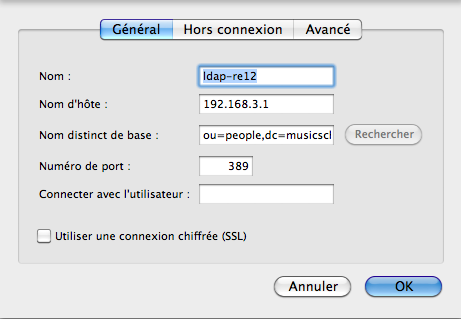
\includegraphics[scale=0.61]{thunderbird-ldap}
\caption{Fenêtre de configuration d'un annuaire dans Thunderbird.}
\label{fig:da}
\end{center}
\end{figure}

Après avoir rentré l'ensemble des informations, chaque utilisateur comportant l'attribut \texttt{mail} dans notre annuaire sera complété automatiquement dans le champ destinataire. Comme les attributs n'étaient pas renseignés, on les ajoute.\\

\begin{lstlisting}[title=ajout-mail.ldif]
dn: sn=Doussot,ou=people,dc=musicschool,dc=fr
changetype: modify
add: mail
mail: doussot@musicschool.fr

dn: sn=Doyen,ou=people,dc=musicschool,dc=fr
changetype: modify
add: mail
mail: doyen@musicschool.fr

dn: sn=Ploix,ou=people,dc=musicschool,dc=fr
changetype: modify
add: mail
mail: ploix@musicschool.fr
\end{lstlisting}


\end{document}